\documentclass{article}

\usepackage[utf8]{inputenc}
\usepackage[brazilian]{babel}
\usepackage{graphicx}
\usepackage{float}
\usepackage[pdftex]{hyperref}
\usepackage{epstopdf}
\usepackage{etoolbox}
\usepackage{amsmath}
\usepackage{amsfonts}
\usepackage{amssymb}
\usepackage{caption}
\usepackage{subcaption}
\usepackage{setspace}
\usepackage{tikz}

\patchcmd{\thebibliography}{\section*}{\section}{}{}
\newcommand{\R}{\ensuremath{\mathbb{R}}}
\newcommand{\Prob}{\ensuremath{\mathbb{P}}}
\newcommand{\K}{\ensuremath{\mathbb{K}}}
\newcommand{\U}{\ensuremath{\mathbb{U}}}
\newcommand{\N}{\ensuremath{\mathbb{N}}}
\newcommand{\Lg}{\ensuremath{\mathbb{L}}}
\newcommand{\T}{\ensuremath{\rm Tr}}
\newcommand{\sg}{{\sigma(x_k)}}

\newcommand{\G}{\ensuremath{\mathcal{G}}}
\newcommand{\F}{\ensuremath{\mathcal{F}}}
\newcommand{\C}{\ensuremath{\mathcal{C}}}
\newcommand{\E}{\ensuremath{\mathcal{E}}}
\newcommand{\Hn}{\ensuremath{\mathcal{H}}}
%\newcommand{\Hoo}{\ensuremath{\mathcal{H}_\infty}}
\newcommand{\Hop}{\ensuremath{\mathcal{H}_{op}}}
% --------------------------------------------------
\newtheorem{theo}{Teorema}
\newtheorem{exa}{Exemplo}
\newtheorem{lemm}{Lema}
\newtheorem{coro}{Corolário}
\newtheorem{defn}{Definição}[section]

%opening


\begin{document}

\begin{titlepage}
\begin{center}

\newcommand{\HRule}{\rule{\linewidth}{0.5mm}}
% Upper part of the page. The '~' is needed because \\
% only works if a paragraph has started.

\includegraphics[width=0.15\textwidth]{logounicamp.pdf}~\\[1cm]

\textsc{\LARGE Universidade Estadual de Campinas}\\[1.5cm]

\textsc{\Large Faculdade de Engenharia Mecânica}\\[0.5cm]

% Title
\HRule \\[0.4cm]
{ \huge \bfseries ES828 - Laboratório de Controle de Sistemas\\ \vspace{1cm} Relatório - Experimento 2 \\
\Large{Método de identificação de plantas eletrônicas} \\[0.4cm] }

\HRule \\[1.5cm]

% Author and supervisor
\begin{minipage}{0.6\textwidth}
\begin{flushleft} \large
\emph{Nome:}\\
Daniel Dello Russo Oliveira\\ Marcelli Tiemi Kian
\end{flushleft}
\end{minipage}
\begin{minipage}{0.2\textwidth}
\begin{flushright} \large
\emph{RA}\\ 101918\\
117892
\end{flushright}
\end{minipage}

\vfill

% Bottom of the page
{\large \today}

\end{center}
\end{titlepage}


\onehalfspacing
\section{Objetivos} 
O objetivo desse experimento o projeto de um controlador Atraso-Avanço que atenda aos requisitos especificados utilizando uma técnica de controle no domínio da frequência. 
	
\section{Projeto do Controlador Atraso-Avanço digital}
Consideramos a planta cuja função de transferência representada pela equação \ref{eq:gs} que foi obtida usando as medidas realizadas durante o experimento 2 \cite{bb:lab2} para o projeto do controlador no formato apresentado pelo roteiro \cite{bb:roteiro} na equação \ref{eq:atav}.\\

\begin{equation}
\label{eq:gs}
G(s) = \frac{\kappa_1*\kappa_2*\kappa_3*\kappa_4}{(s*\tau_2 + 1)(s*\tau_3 + 1)s}
\end{equation}

\begin{table}[H]
\centering
\caption{Parâmetros numéricos da função de transferência}
\label{tab:valores}
\begin{tabular}{|c|c|}
	\hline Parâmetro & Valor \\ 
	\hline $\kappa_1$ & $-0.1005$\\ 
	\hline $\kappa_2$ & $-2.1508$\\ 
	\hline $\kappa_3$ & $-4.6448$\\ 
	\hline $\kappa_4$ & $-5.6307$\\ 
	\hline $\tau_2$ & $0.0210$\\ 
	\hline $\tau_3$ & $0.0244$ \\ 	
	\hline 
\end{tabular} 
\end{table}

\begin{equation}
\label{eq:atav}
C(s)=\kappa \frac{\alpha_v \tau_v s + 1}{\tau_v s + 1} \frac{\alpha_t \tau_t s + 1}{\tau_t s + 1}
\end{equation}

\subsection{Requisitos do Sistema e Projeto}
Seguindo o proposto no roteiro \cite{bb:roteiro} as especificações do sistema são:
\begin{itemize}
	\item Erro em regime permanente a uma entrada rampa de $2\%$.
	\item Margem de fase de pelo menos $45^o$.
	\item Sobrelevação de no máximo $20\%$ para uma entrada degrau.
	\item Amplitude do sinal de controle não pode ultrapassar $\pm10$ [Volts].
\end{itemize}\

Utilizando a metodologia indicada no roteiro\cite{bb:roteiro}, iniciamos o cumprimento do primeiro requisito considerando o controlador $C(s)=\kappa$ e encontramos este valor para que o erro a uma entrada rampa seja de $2\%$. Para isso, utilizamos o teorema do valor final: 
\begin{equation}
\lim_{t\to\infty}e(t)=\lim_{s\to0}sE(s) = \lim_{s\to0}\frac{s}{s^2(1+\kappa G(s))}
\end{equation}

Chegamos então a: 
\begin{equation}
	\kappa=\frac{50}{\kappa_1 \kappa_2 \kappa_3 \kappa_4}
\end{equation}

Posteriormente, para os requisitos de margem de fase e sobrelevação (ambos ligados ao fator de amortecimento do sistema), calculamos a margem de fase de $\kappa G(s)$ dada por $M_f=17.4123$, menor que margem de fase mínima de $45^o$. Como margem de segurança, adotaremos as margens de fase desejadas de $M_{d1}=45^o$, $M_{d2}=50^o$ e $M_{d3}=55^o$ que também garantem sobrelevação menor que $20\%$. Projetamos três controladores de maneira a ter opções caso a implementação real do sistema não corresponda às simulações. Idealmente gostaríamos de adotar uma margem de fase mais elevada, porém, após comparar a sua resposta com a resposta do sistema com margem de $45^o$, decidimos implementar mais opções.

A partir destas margens de fase encontramos os parâmetros $\alpha_v$ dos controladores utilizando as equações \ref{eq:phi} e \ref{eq:av}. Com o conhecimento de $\alpha_v$ e da frequência $\omega_g$ na qual $\mod{\kappa G(j\omega_g)}=\sqrt{\alpha_v}$, encontramos $\tau_v$ pela equação \ref{eq:tv}. Os parâmetros $\alpha_t$ e $\tau_t$ são calculados pelas equações \ref{eq:at} e \ref{eq:tt}

\begin{equation}
\label{eq:phi}
\phi=M_d-M_f
\end{equation}
\begin{equation}
	\label{eq:av}
	\alpha_v=\frac{1+\sin{\phi}}{1-\sin{\phi}}
\end{equation}
\begin{equation}
	\label{eq:tv}
	\tau_v=\frac{1}{\omega_g \sqrt{\alpha_v}}
\end{equation}
\begin{equation}
\label{eq:at}
\alpha_t=\frac{1}{\alpha_v}
\end{equation}
\begin{equation}
\label{eq:tt}
\tau_t=10\frac{\alpha_v \tau_v}{\alpha_t}
\end{equation}

Logo, a função de transferência dos controladores são dadas pela equação \ref{eq:contr1} e seus parâmetros pela tabela \ref{tab:contr}.

\begin{equation}
\label{eq:contr}
C(s)=\kappa \frac{\alpha_v \tau_v s + 1}{\tau_v s + 1} \frac{\alpha_t \tau_t s + 1}{\tau_t s + 1}
\end{equation}

\begin{table}[H]
	\centering
	\caption{Parâmetros numéricos da função de transferência dos controladores Avanço-Atraso}
	\label{tab:contr}
	\begin{tabular}{|c|c|c|c|}
		\hline Parâmetro & Controlador 1& Controlador 2& Controlador 3 \\ 
		&$M_d = 45^o$&$M_d = 50^o$&$M_d = 55^o$\\
		\hline $\kappa$ & $8.8445$ & $8.8445$ & $8.8445$\\ 
		\hline $\alpha_v$ & $2.7251$ & $3.3345$ & $4.1279$\\ 
		\hline $\tau_v$ & $0.0257$ & $0.0250$ & $0.0243$\\ 
		\hline $\alpha_t$ & $0.3670$ & $0.2999$ & $0.2423$\\ 
		\hline $\tau_t$ & $1.9108$ & $2.7768$ & $4.1334$\\ 
		\hline 
	\end{tabular} 
\end{table}

\subsection{Simulação e Comparação}
Com o auxílio do Simulink simulamos as respostas dos 3 controladores à uma onda quadrada de amplitude $1V$ e frequência de $0,25Hz$, que podem ser vistas nas figuras \ref{fig:yr45}, \ref{fig:yr50} e \ref{fig:yr55}, e os seus esforços de controle, mostrados nas figuras \ref{fig:ur45}, \ref{fig:ur50} e \ref{fig:ur55}.
\begin{figure}[H]
	\centering
	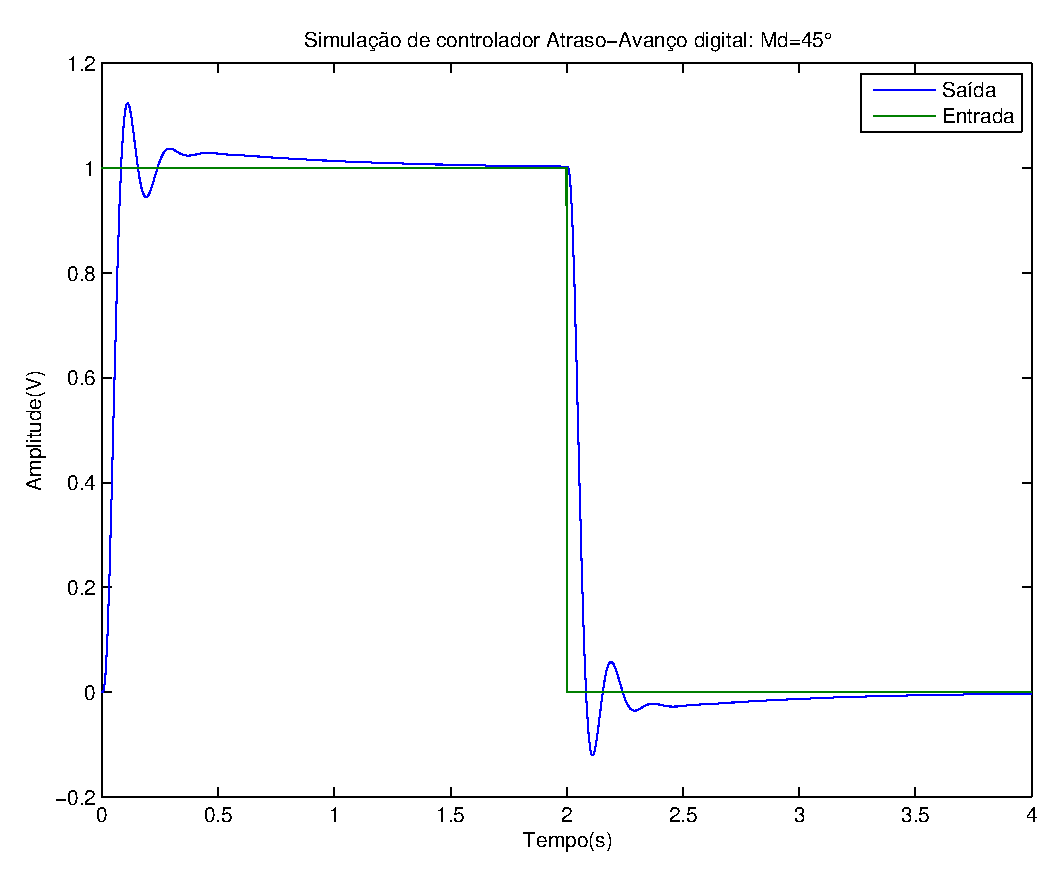
\includegraphics[width=0.8\linewidth]{yr45}
	\caption{Resposta à onda quadrada do controlador projetado para margem de fase de $45^o$}
	\label{fig:yr45}
\end{figure}
\begin{figure}[H]
	\centering
	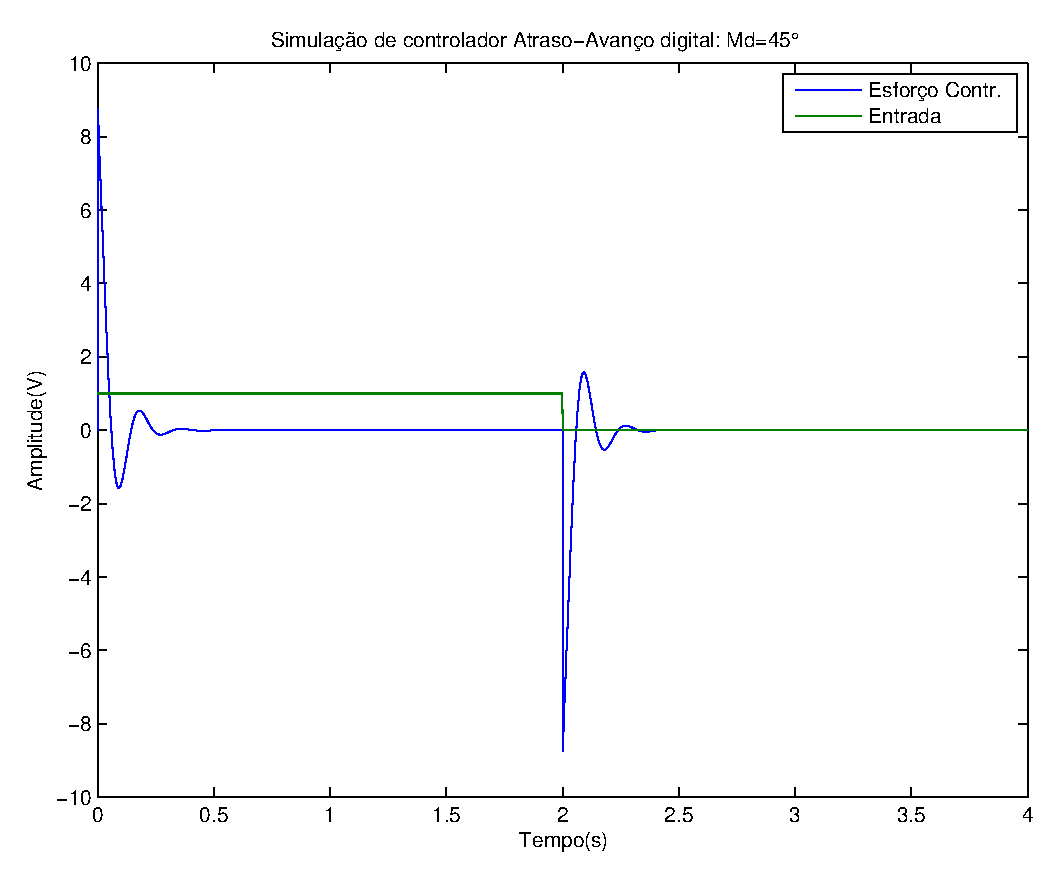
\includegraphics[width=0.8\linewidth]{ur45}
	\caption{Esforço de controle para onda quadrada do controlador projetado para margem de fase de $45^o$}
	\label{fig:ur45}
\end{figure}

\begin{figure}[H]
	\centering
	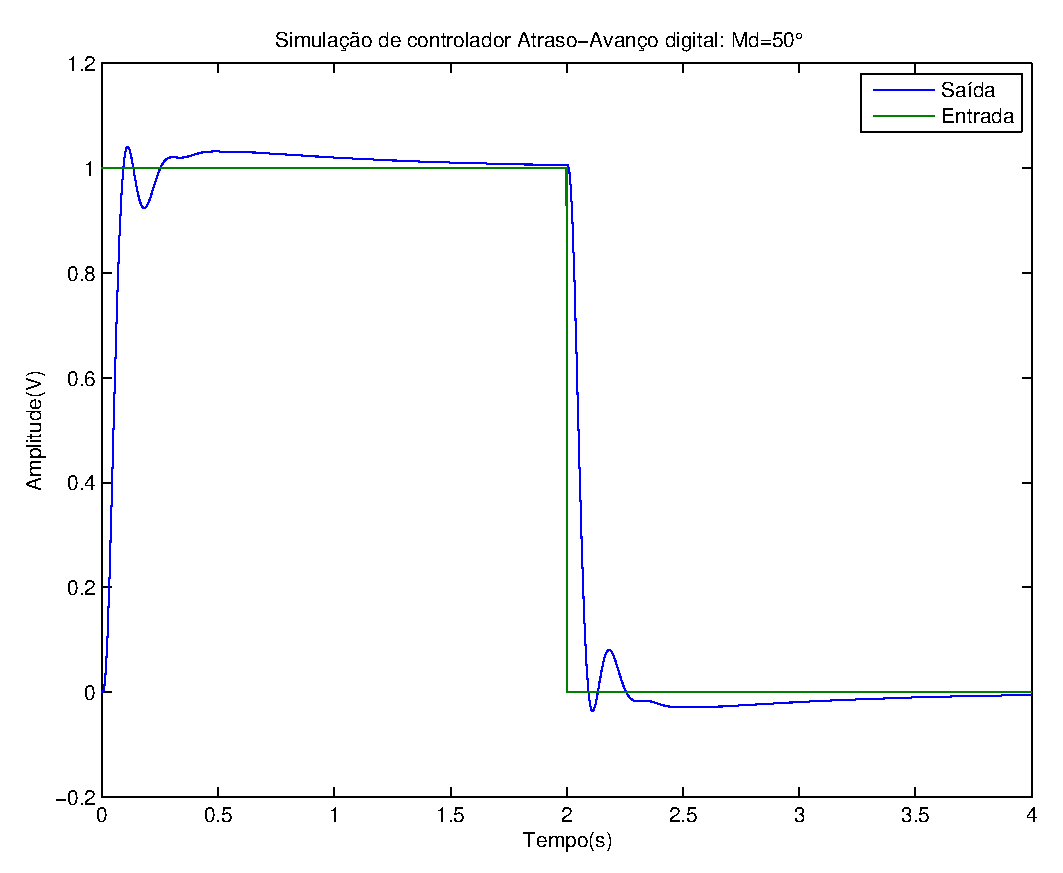
\includegraphics[width=0.8\linewidth]{yr50}
	\caption{Resposta à onda quadrada do controlador projetado para margem de fase de $50^o$}
	\label{fig:yr50}
\end{figure}
\begin{figure}[H]
	\centering
	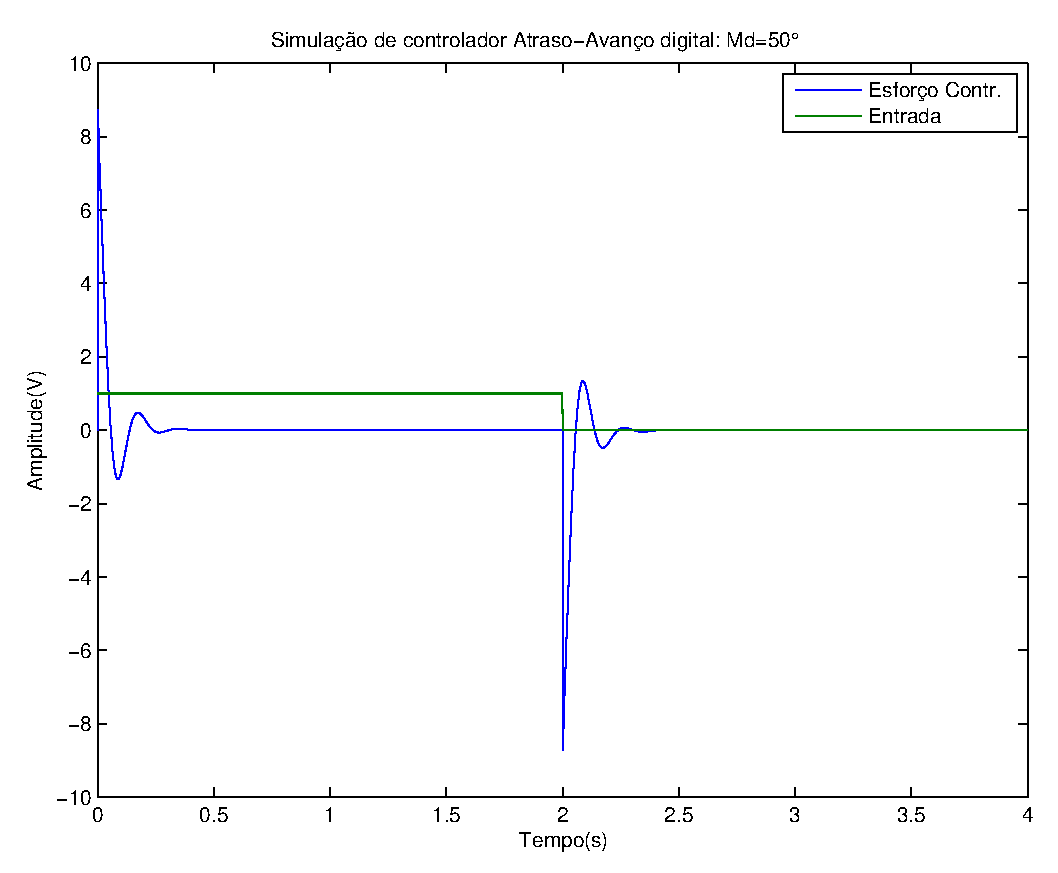
\includegraphics[width=0.8\linewidth]{ur50}
	\caption{Esforço de controle para onda quadrada do controlador projetado para margem de fase de $50^o$}
	\label{fig:ur50}
\end{figure}


\begin{figure}[H]
	\centering
	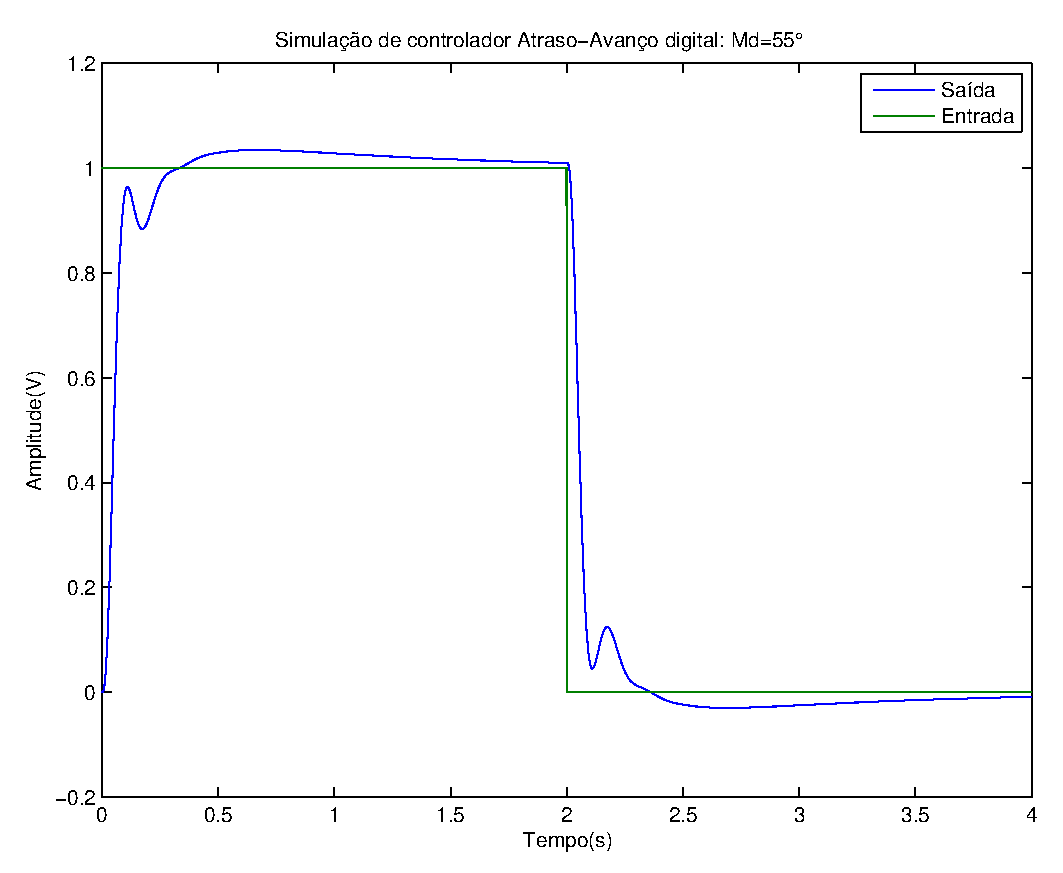
\includegraphics[width=0.8\linewidth]{yr55}
	\caption{Resposta à onda quadrada do controlador projetado para margem de fase de $55^o$}
	\label{fig:yr55}
\end{figure}
\begin{figure}[H]
	\centering
	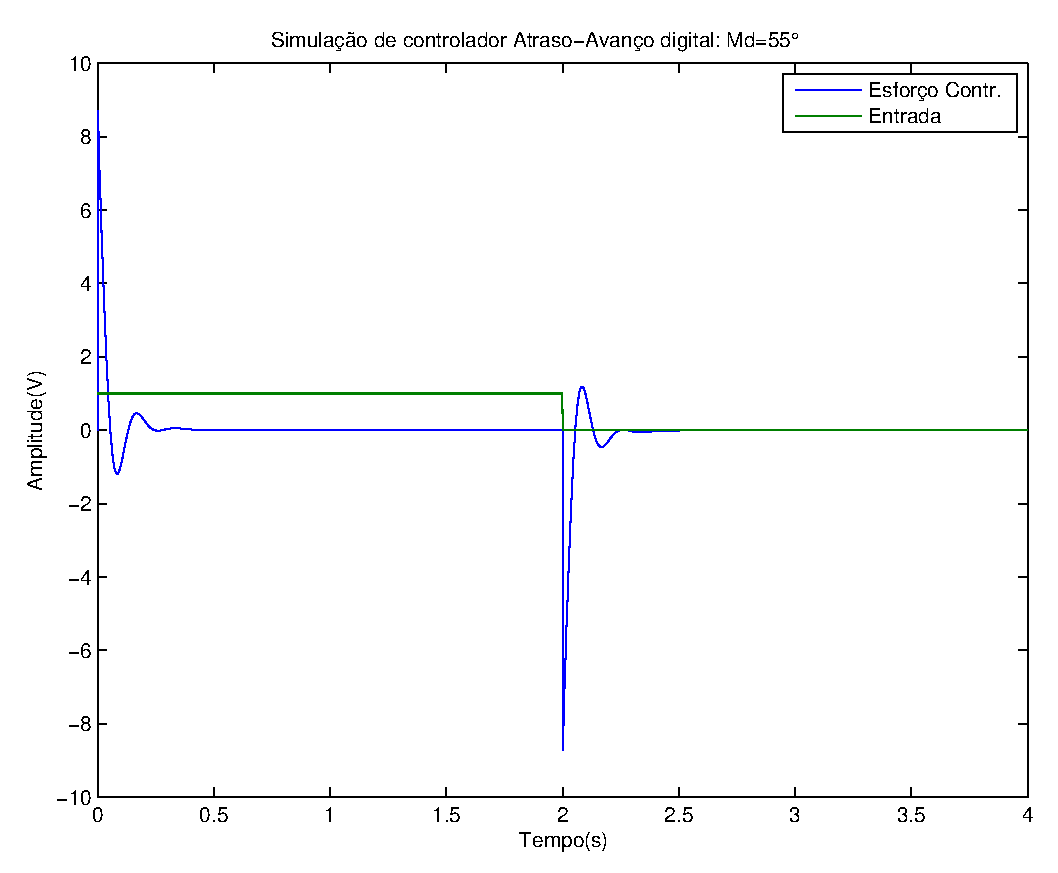
\includegraphics[width=0.8\linewidth]{ur55}
	\caption{Esforço de controle para onda quadrada do controlador projetado para margem de fase de $55^o$}
	\label{fig:ur55}
\end{figure}

Simulamos também as respostas destes controladores à uma rampa, estas são mostradas nas figuras \ref{fig:yru45r},\ref{fig:yru50r} e \ref{fig:yru55r}. Como podemos ver, o erro estacionário para essa entrada é próxima de $2\%$ para todos os controladores, conforme desejado.
\begin{figure}[H]
	\centering
	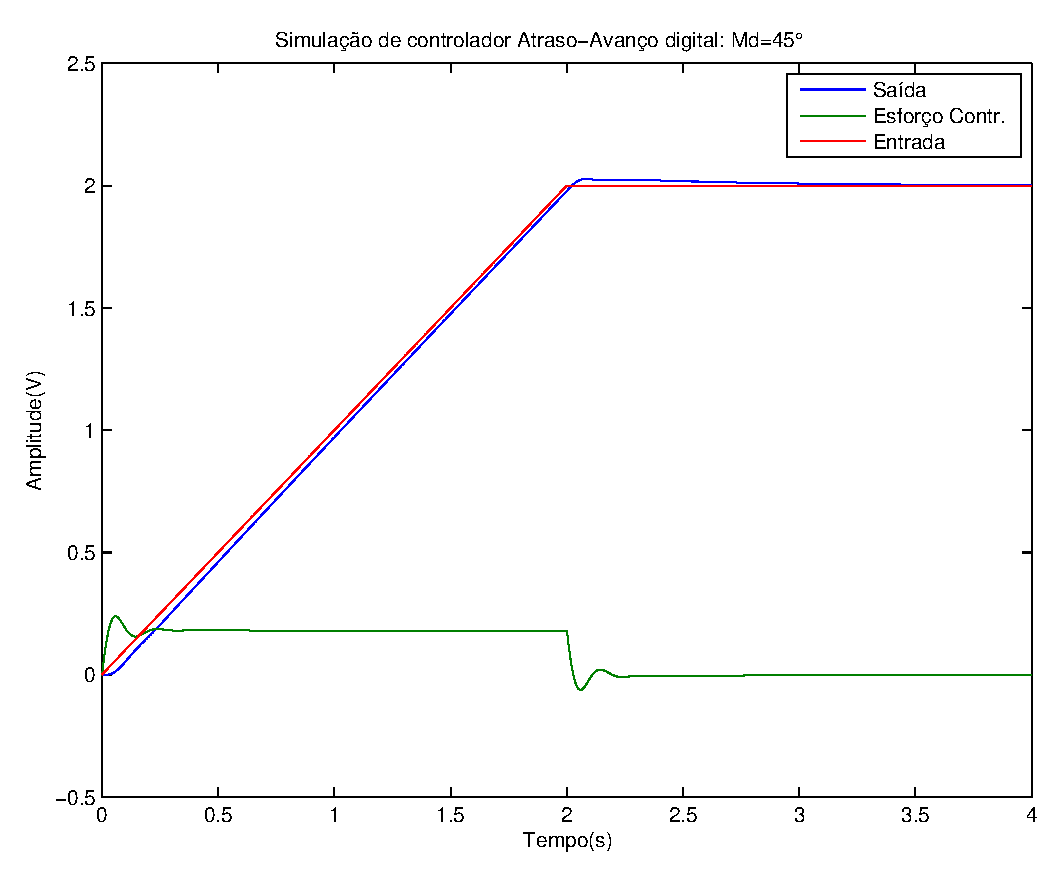
\includegraphics[width=0.8\linewidth]{yur45r}
	\caption{Resposta à rampa do controlador projetado para margem de fase de $45^o$}
	\label{fig:yru45r}
\end{figure}
\begin{figure}[H]
	\centering
	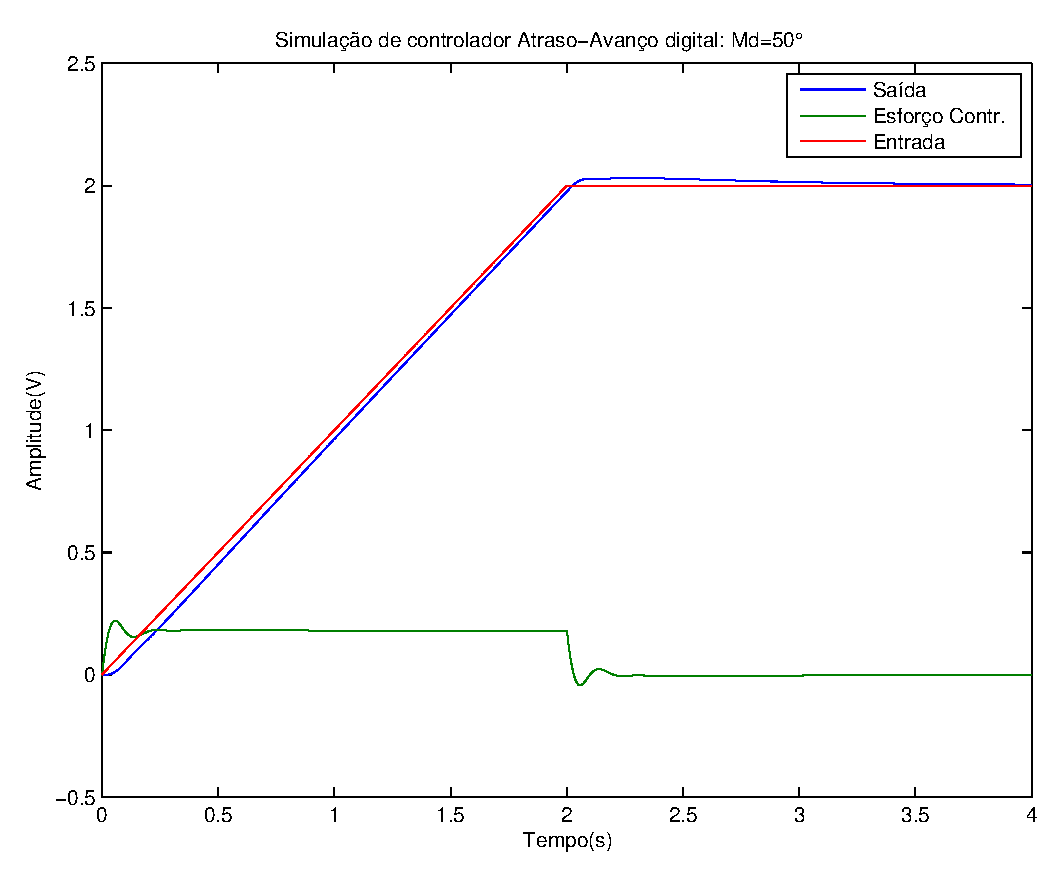
\includegraphics[width=0.8\linewidth]{yur50r}
	\caption{Resposta à rampa do controlador projetado para margem de fase de $50^o$}
	\label{fig:yru50r}
\end{figure}
\begin{figure}[H]
	\centering
	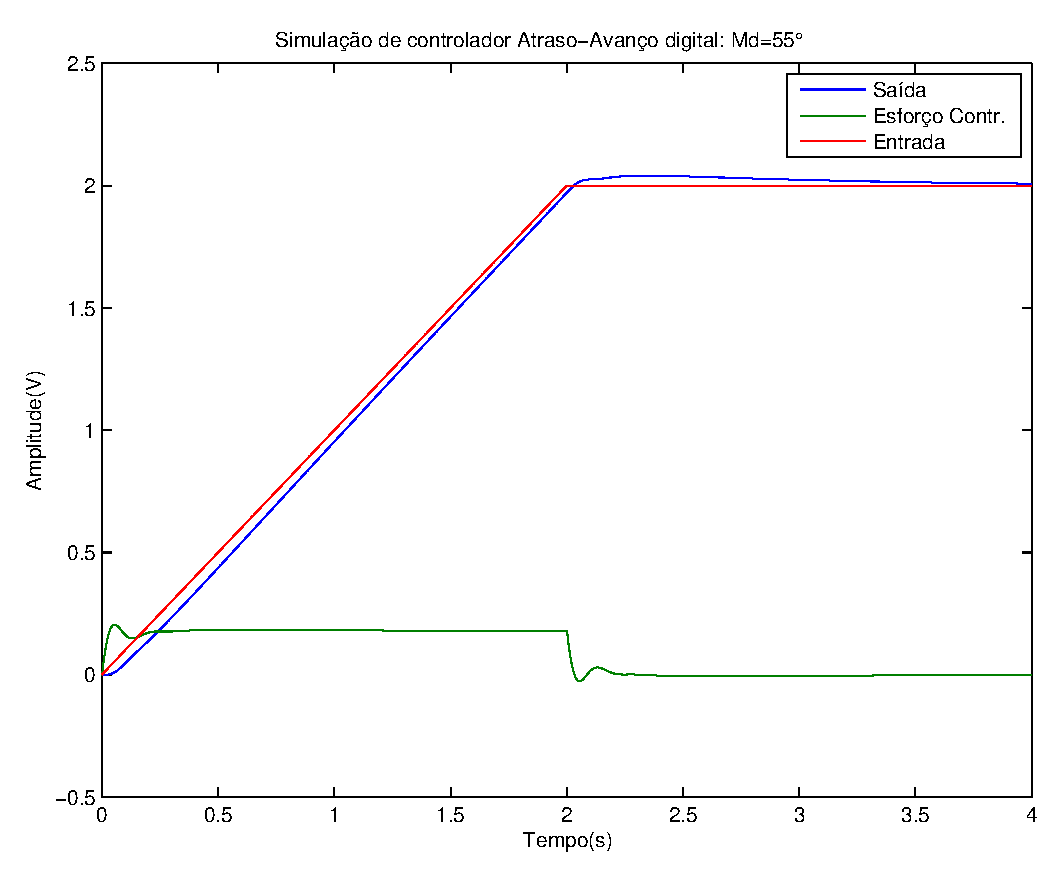
\includegraphics[width=0.8\linewidth]{yur55r}
	\caption{Resposta à rampa do controlador projetado para margem de fase de $55^o$}
	\label{fig:yru55r}
\end{figure}

O controlador com margem de fase de $45^o$ é o que apresenta o menor tempo de estabilização e erro estacionário. Porém os outros controladores não apresentam a sobrelevação relativamente elevada que o primeiro controlador apresenta. A tabela \ref{tab:avat} apresenta as características das respostas desses controladores, obtida com o auxílio da função \textit{stepinfo} do Matlab.
\begin{table}[H]
	\centering
	\caption{Características da resposta dos controladores Avanço-Atraso Simulados}
	\label{tab:avat}
	\begin{tabular}{|c|c|c|c|}
		\hline Características & Controlador 1& Controlador 2& Controlador 3 \\ 
		&$M_d = 45^o$&$M_d = 50^o$&$M_d = 55^o$\\
		\hline Sobrelevação & $12.3698\%$ & $4.0867\%$ & $3.4618\%$\\ 
		\hline Tempo de estabilização & $0.7454s$ & $1.0142s$ & $1.3472s$\\ 
		\hline Tempo de subida & $0.0503s$ & $0.0553s$ & $0.0628s$\\ 
		\hline Erro estacionário (degrau) & $0.3\%$ & $0.6\%$ & $1\%$\\ 
		\hline Erro estacionário (rampa) & $2\%$ & $2.5\%$ & $3\%$\\ 
		\hline 
	\end{tabular} 
\end{table}

Comparamos esse controlador com os controladores projetados no durante o pré relatório do experimento 3 \cite{bb:prelab3}. Para o controlador PID projetado com SISO Tool, cuja performance pode ser vista nas figuras \ref{fig:stepgkscl}, \ref{fig:rampgkscl} e o controlador proporcional projetado para obter o menor tempo de estabilização, cuja performance pode ser vista nas figuras \ref{fig:stepgkocl} e \ref{fig:rampgkocl}.

\begin{figure}[H]
	\centering
	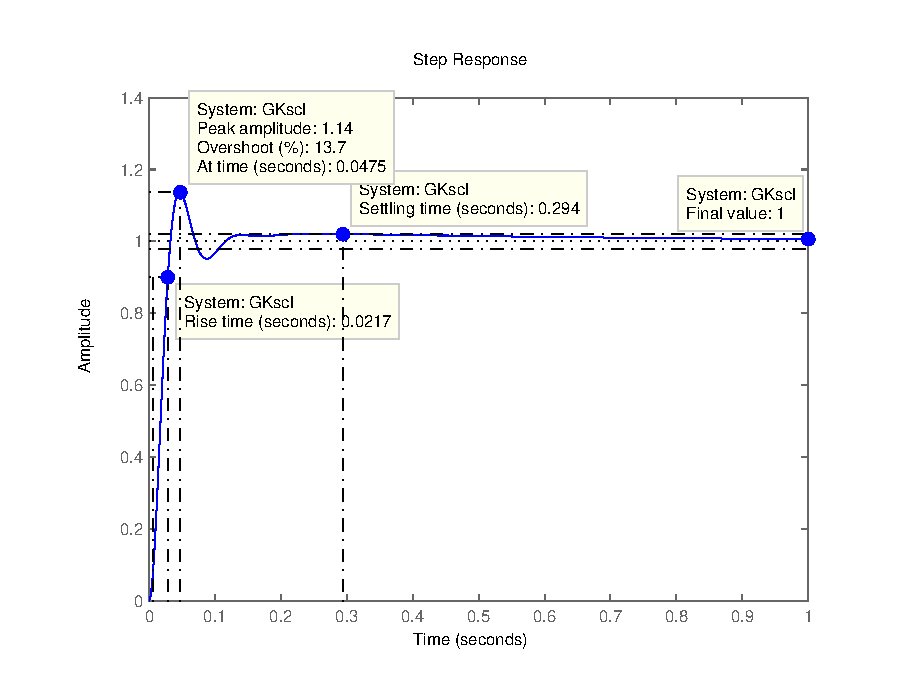
\includegraphics[width=0.8\linewidth]{stepgkscl}
	\caption{Resposta ao degrau para o sistema com controlador PID projetado com o auxílio do SISOTool}
	\label{fig:stepgkscl}
\end{figure}
\begin{figure}[H]
	\centering
	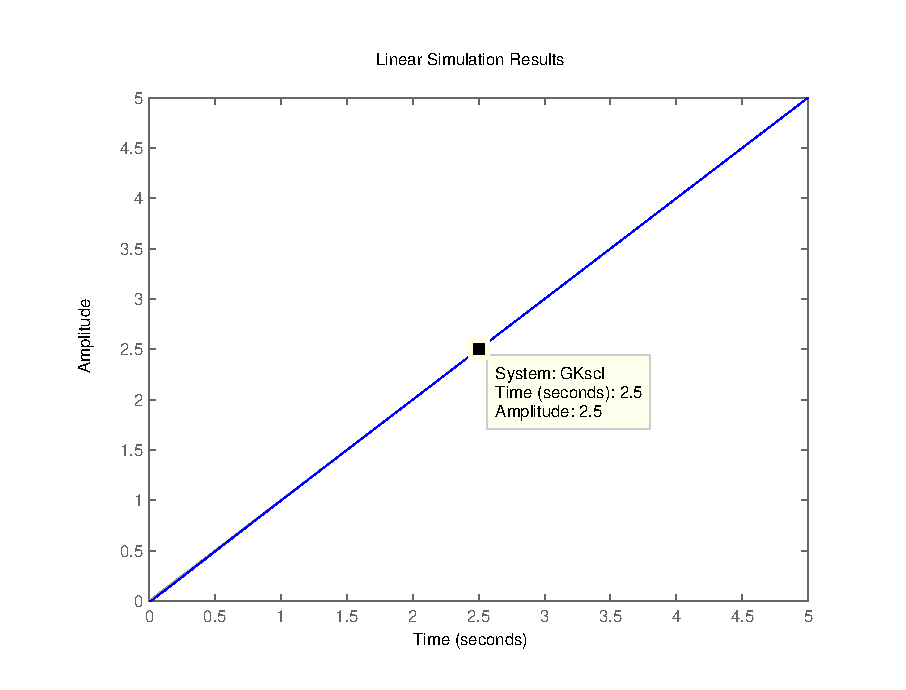
\includegraphics[width=0.8\linewidth]{rampgkscl}
	\caption{Resposta à rampa para o sistema com controlador PID projetado com o auxílio do SISOTool}
	\label{fig:rampgkscl}
\end{figure}

 \begin{figure}[H]
 	\centering
 	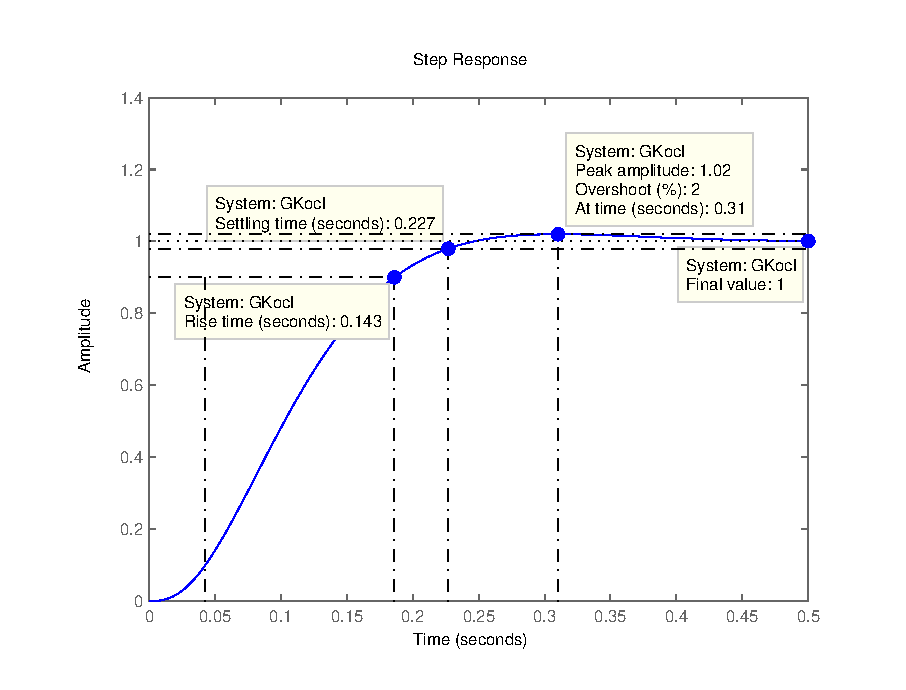
\includegraphics[width=0.8\linewidth]{stepgkocl}
 	\caption{Resposta ao degrau do sistema com controlador proporcional}
 	\label{fig:stepgkocl}
 \end{figure}
 
 \begin{figure}[H]
 	\centering
 	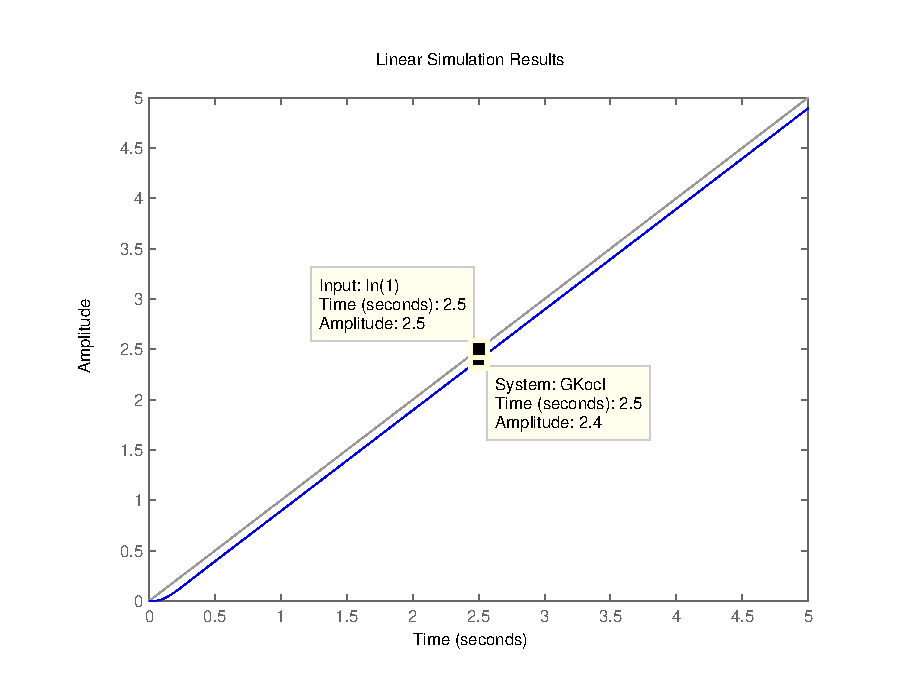
\includegraphics[width=0.8\linewidth]{rampgkocl}
 	\caption{Resposta à rampa do sistema com controlador proporcional}
 	\label{fig:rampgkocl}
 \end{figure}
 
 Como podemos perceber os controladores Avanço-Atraso apresentam uma resposta mais lenta que os controladores PID e proporcional. Porém suas respostas à rampa apresentam um erro estacionário significativamente menor que o controlador proporcional e sabemos que a margem de fase do sistema é maior para esse controlador que ela é para o PID projetado pelo SISOTool. Embora o controlador PID tenha apresentado um desempenho simulado significativamente melhor, sabemos que quando implementado o mesmo foi inferior, logo não podemos comparar efetivamente ambos os controladores sem antes implementá-los.
 
\begin{thebibliography}{widestlabel}
	\bibitem{bb:roteiro}{Roteiro do experimento disponibilizado para os alunos}
	\bibitem{bb:prelab3}{KIAN, Marcelli; OLIVEIRA, Daniel. \textit{Pré Relatório - Experimento 3:} Controle de plantas eletrônicas utilizando um controlador PID digital.}
	\bibitem{bb:lab2}{KIAN, Marcelli; OLIVEIRA, Daniel. \textit{Relatório - Experimento 2:} Identificação de plantas eletrônicas.}
\end{thebibliography}
\end{document}

